\documentclass[11pt]{report}
% define the title
\usepackage[brazil]{babel}
\usepackage[utf8]{inputenc}		%Usar acentos diretos do teclado
\usepackage[T1]{fontenc}		%Padrão para imagens
\usepackage{graphicx}
\usepackage{subfigure}
\usepackage{rotating}
\usepackage{longtable}
\usepackage{amsmath}
\usepackage{amsfonts}
\usepackage{amssymb}
\usepackage{geometry}
\usepackage{caption}
\geometry{left=3cm, right=2cm, top=2cm, bottom=2cm}
% Title Page
\title{Lista de Exercícios 1 - Sistemas Não Lineares - Fenômenos e Exemplos de Não-Linearidades}
\author{Pedro Yochinori Gushiken}



\begin{document}
\maketitle
\chapter{Sistemas que cumprem os requisitos listados}
\section{Viola o Princípio da Superposição, Forças de Arraste}
Um exemplo de sistema não linear que não segue o princípio da superposição é o de uma massa esférica sendo acelerada por uma força constante dentro de alguma espécie de fluido (Equação do Arraste no equilíbrio dinâmico). A medida que a velocidade do corpo aumenta, a resultante das forças de arraste agindo sobre o corpo aumenta proporcionalmente ao quadrado da velocidade até que o corpo atinja um equilíbrio de forças numa certa velocidade terminal. Para duas forças diferentes aplicadas sobre o mesmo corpo ao mesmo tempo é possível observar que a velocidade terminal não será igual a soma das velocidades terminais que seriam adquiridas caso as forças fossem aplicadas de forma isolada. A densidade $\rho$ do fluido é de $1g/{cm}^3$, a área de superfície de contato do objeto é de $1m^2$, o coeficiente de arraste para uma esfera é de 0.47 adimensional e a massa do corpo é de $1kg$.
\section{Escape em Tempo Finito, Estimador de Parâmetros via Regra do MIT}

Um exemplo de sistema não linear que exibe a propriedade de escape em tempo é o estimador de parâmetros que segue a regra do MIT. Dependendo da calibragem dos ganhos adaptativos $\gamma$ é possível observar o fenômeno do escape em tempo finito. Usamos como base um estimador construído para um sistema RL simples, usando leis adaptativas $\theta_1 = \gamma_1 e_0 u$ e $\theta_2 = -\gamma_2 e_0 y$, onde a saída y corresponde a corrente que passa pelo circuito e a entrada u à tensão imposta na entrada. A resistência corresponde $R=1.2\Omega$, indutância $L=0.1mH$, ganhos $\gamma_1=1e6$, $\gamma_2=20$ e estimativas iniciais $\theta_1(0)=45$ e $\theta_2(0)=80$.
\section{Múltiplos Pontos de Equilíbrio, Câmara de vácuo térmica}
Retiramos a modelagem da temperatura de entrada e saída de uma Câmara de Vácuo-Térmico da introdução do livro sobre identificação de parâmetros do professor Aguirre. Escolhemos arbitrariamente uma temperatura de entrada de 1K e confirmamos através de simulação com diferentes condições iniciais que a equação escolhida possui pelo menos dois pontos de equilíbrio distintos. A equação modelada é $\dot{y}=2.13\times 10^{-12} u^4 - 2.41\times 10^{-12} y^4 + 3.46\times 10^{-10} y^3 - 2.63\times 10^{-10} y^2 u$.

\section{Ciclo Limite, Temperatura numa sala vazia e refrigerada}
Um exemplo de fenômeno do ciclo limite, quando um sistema converge para uma oscilação com frequência constante, pode ser a temperatura de uma sala refrigerada por um sistema de ar condicionado que liga para uma determinada temperatura e desliga com outra distinta. Normalmente isto é implementado através de um sistema de agulha e contator, porém na simulação representamos isto através de um relé com histerese. Para condições iniciais distintas, o sistema converge para uma oscilação com frequência constante em torno de um certo valor de temperatura. Modelamos a sala recebendo uma potência externa fixa de 300 unidades arbitrárias, enquanto o ar condicionado retira uma potência de 200 unidades arbitrárias e liga para uma temperatura acima de 290K, desligando para temperaturas abaixo de 287K.  Uma unidade arbitrária multiplicada por tempo produz 1 Kelvin. Simulamos o sistema para uma temperatura inicial de 250K e 320K.

\section{Caos e Bifurcação, Circuito de Chua}

Simulamos um circuito de Chua, que exibe o fenômeno do Caos e também o da Bifurcação. Para a Bifurcação uma mudança quantitativa nos parâmetros do sistema, pode aparecer uma mudança qualitativa no comportamento, como vemos nas primeiras duas figuras. O fenômeno do Caos indica que para uma mudança arbitrariamente pequena nas condições iniciais, a evolução do comportamento do sistema pode ser drasticamente diferente, como vemos nas duas figuras seguintes. Intuitivamente é possível notar que os dois fenômenos são semelhantes, enquanto o Caos lida com condições iniciais, a bifurcação lida com os parâmetros. Para confirmar o fenômeno do Caos simulamos o circuito para uma corrente inicial no indutor $L_1$ $I_i=2A$, tensão inicial no capacitor $C_1$ $V_{c1}=2V$, tensão no capacitor $C_2$ $V_{c2}=0V$ e para condições iniciais diferentes mas arbitrariamente próximas corrente inicial no indutor $L_1$ $I_i=2A$, tensão inicial no capacitor $C_1$ $V_{c1}=2V$, tensão no capacitor $C_2$ $V_{c2}=0.01V$. O valor dos resistores R é de $12\Omega$, dos resistores $R_A=12\Omega$, dos capacitores $C_1=1mF$ e $C_2=0.1mF$ e do indutor $L_1=1mH$. 

Para o fenômeno da Bifurcação simulamos o circuito com os valores dados acima e também com valores arbitrariamente próximos R=$12\Omega$, $R_A=12\Omega$, $C_1=1mF$ e $C_2=0.101mF$, $L_1=1mH$. Notar a diferença entre a variável VC2-1 e a variável VC2-2 nos gráficos.


\section{Salto, Sistema massa mola com ressonância}
Embora não recomendado na lista, utilizamos o exemplo exposto no livro Dinâmica Não-Linear e Caos, do autor Marcelo Amorim Savi. O exemplo consiste de uma sistema massa mola não linear com ponto de contato com outro sistema massa mola que altera as propriedades do sistema, de modo que para uma determinada faixa de frequências a ressonância faz com que o primeiro sistema massa mola "encaixe" no segundo sistema, fazendo com que a amplitude de oscilação diminua drasticamente e o sistema fique "colado". Simulamos o sistema para uma frequência $\Omega$ de 0.7, 1.1 e 1.5 radianos por segundo. A equação que governa o sistema normalmente é $\ddot{u} + w_0^2 u + 2\xi w_0 \dot{u} = \mu cos(\Omega t)$, mas para $u \geq 0.8$ (alteramos esse valor na equação dada pelo livro) temos $\ddot{u} + w_0^2 u + w_s^2 (u-0.8) + 2(\xi w_0 +2\xi_s w_s)\dot{u} = \mu cos(\Omega t)$. Usamos os valores de $w_0 = 1, w_s=3.16, \xi_s=0.0475, \xi = 0.025 $. Observamos que para um sistema que esteja operando numa região próxima a u=0.8, a introdução de uma pequena perturbação pode mudar a equação que rege o comportamento. 

\section{Controlador PI não linear}
Simulamos um sistema controlado por um controlador linear do tipo PI e o mesmo sistema controlado por um PI não-linear com um termo proporcional ao cubo do erro. A planta a ser controlada tem função de transferência $G(s)= \frac{1}{s^2+8s+1}$, deixamos os PIs com constantes $K_p=1, K_i=1$ "de fábrica" pois queremos apenas fazer a comparação de desempenho entre os o controle linear e o não linear. Introduzimos uma referência r=10.

\section{Controle com Relé, VS-MRAC}

Implementamos um controlador adaptativo por modelo de referência e estrutura variável para um sistema instável de primeira ordem (VS-MRAC). A lei adaptativa foi implementada sem histerese (função sinal, desempenhada por relé) e com histerese. Notamos que a frequência do chattering diminui de acordo com os valores escolhidos para histerese, com um tradeoff em termos da amplitude de oscilação do sistema em torno do valor de referência. O sistema controlado é a planta com função de transferência instável $G(s) = \frac{1}{s-1}$, o modelo de referência é $\frac{1}{s+1}$ e o valor escolhido de $\bar{\theta}$ para ambas as variáveis é de 500. 



\section{Condição de Lipschitz Local e Condição de Lipschitz Global}
Um sistema não linear que é globalmente Lipschitz é a equação $\dot{x}=f(x)=sen(e^{sen(x)})$, pois o valor da função f(x) é regido pelo seno de uma função que é contínua e limitada, sua constante de Lipschitz é igual ao valor máximo de f(x) que é 1. Um sistema não linear que é localmente Lipschitz é o sistema governado pela equação $\dot{u}=u^2$ se  $u\leq 4 \wedge u\geq-4$ , $\dot{u}=0$ se $u\leq-4$ e
$\dot{u}=-4$ se $u\geq4$. Para $u\leq-4 \vee u\geq4$ a constante de Lipschitz do sistema é 0 pois f(x) é uma constante, e para $u\leq 4 \wedge u\geq-4$ a constante de Lipschitz do sistema é 8 que é o valor máximo da derivada de f(x).


\chapter{Figuras}
 \begin{figure}[htpb!]
  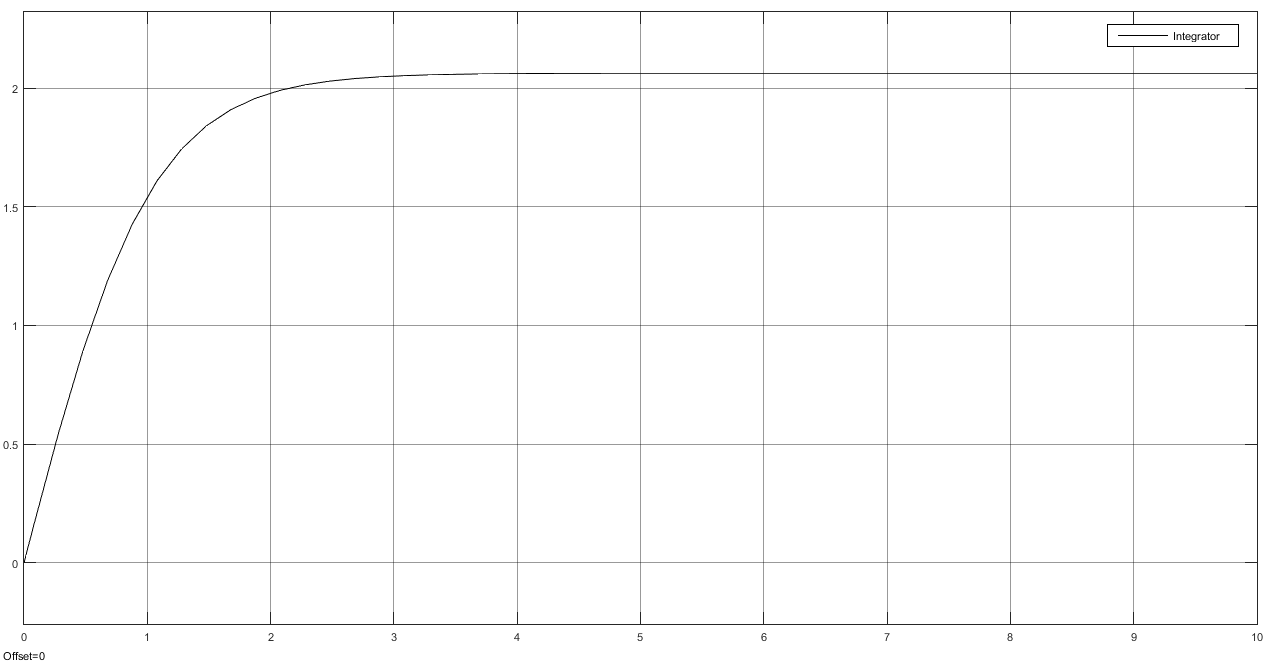
\includegraphics[width=.5\linewidth]{FArrasteV1.png}
  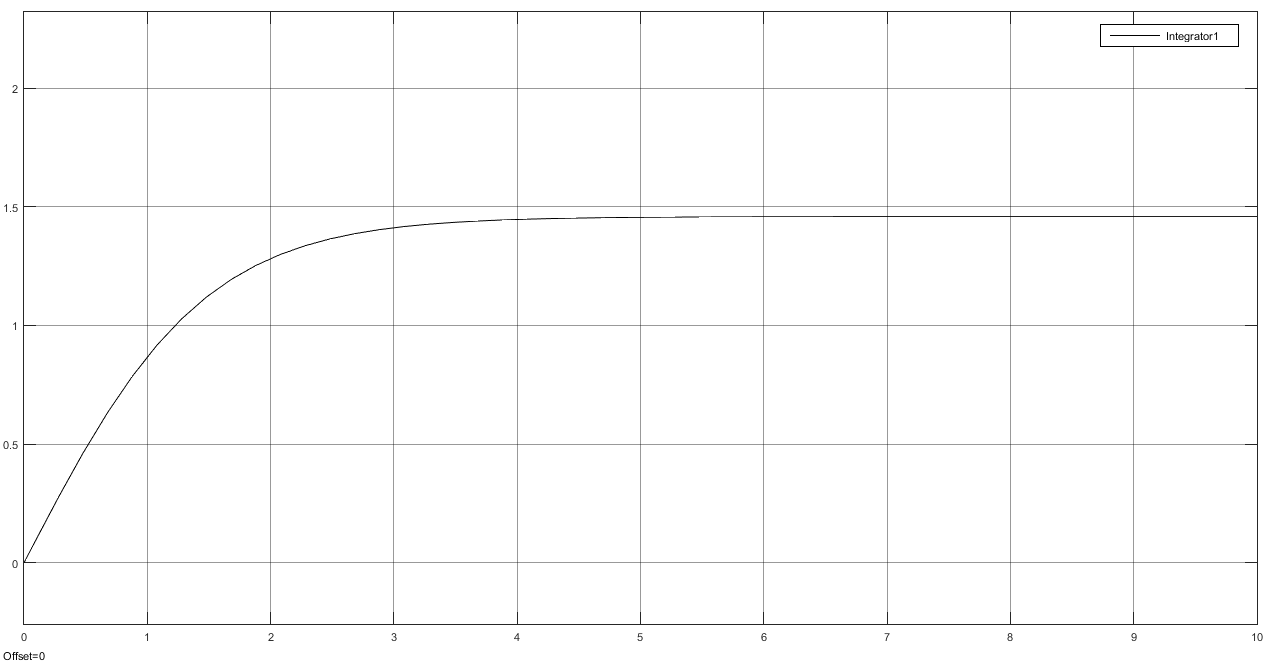
\includegraphics[width=.5\linewidth]{FArrasteV2.png}
  \caption{a)Velocidade adquirida para um Força de 2N b)Velocidade adquirida para um Força de 1N}
  \end{figure}
 
 
 
 \begin{figure}[htpb!]
 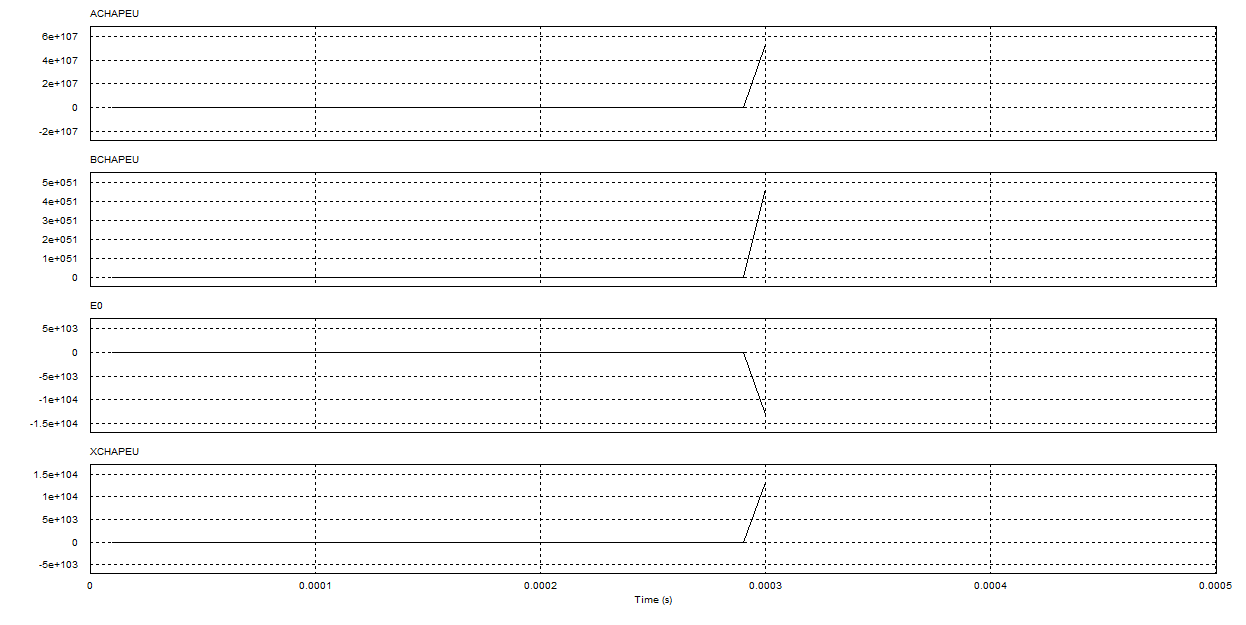
\includegraphics[width=\linewidth]{EscapeTempoFinitoVariaveis.png}
 \caption{Fenômeno do Escape em Tempo Finito}
 \end{figure}
 

\begin{figure}[htpb!]
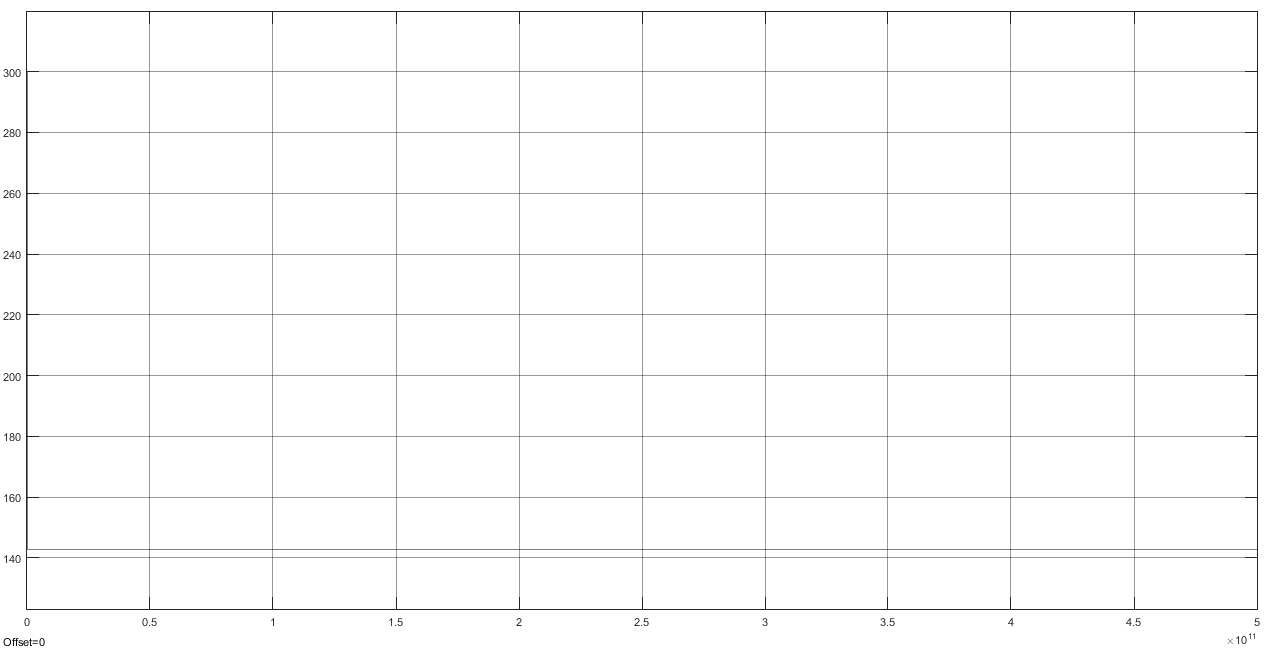
\includegraphics[width=.5\linewidth]{MultEqTemp1.png}
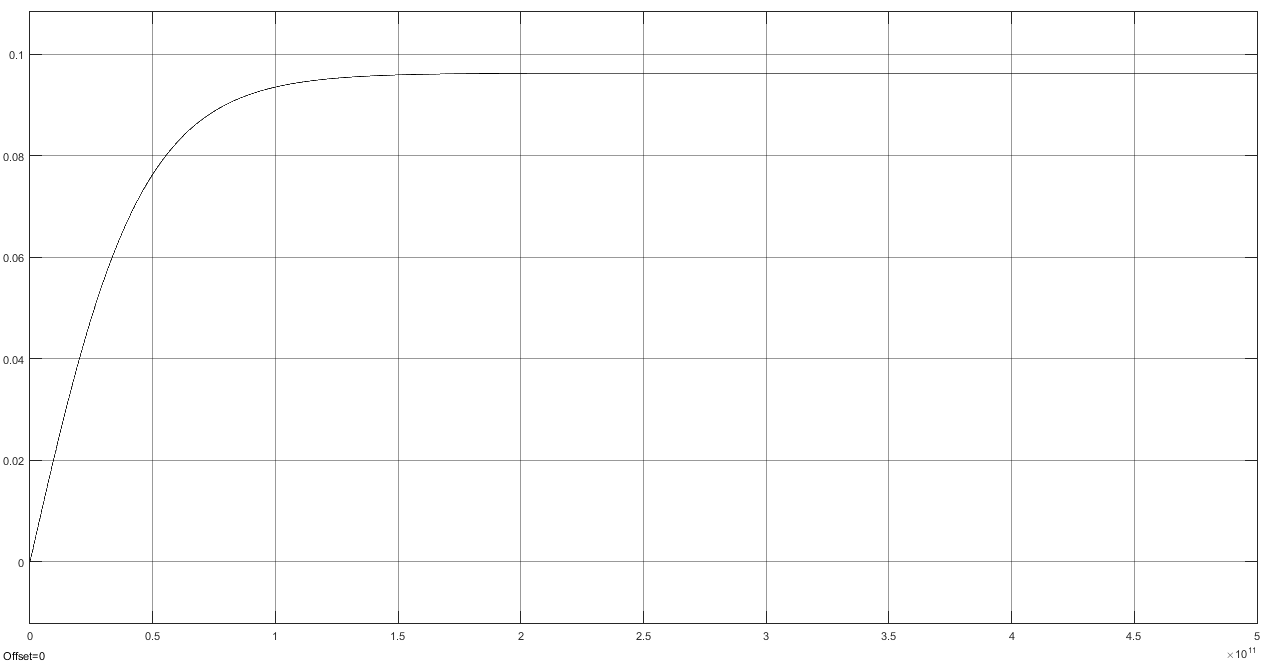
\includegraphics[width=.5\linewidth]{MultEqTemp2.png}
\caption{a)Gráfico da temperatura de saída para uma condição inicial y(0)=300K b)Gráfico da temperatura de saída para uma condição inicial y(0)=0K}
\end{figure}


\begin{figure}[htpb!]
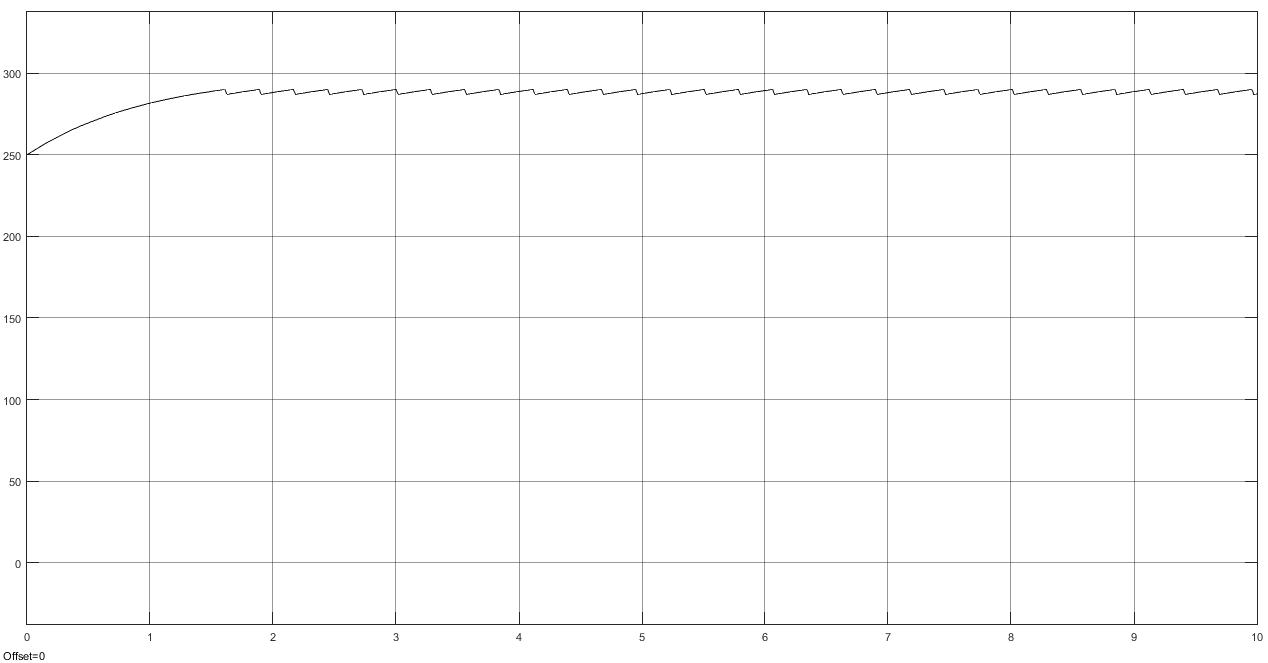
\includegraphics[width=.5\linewidth]{CicloLimiteTemp1.png}
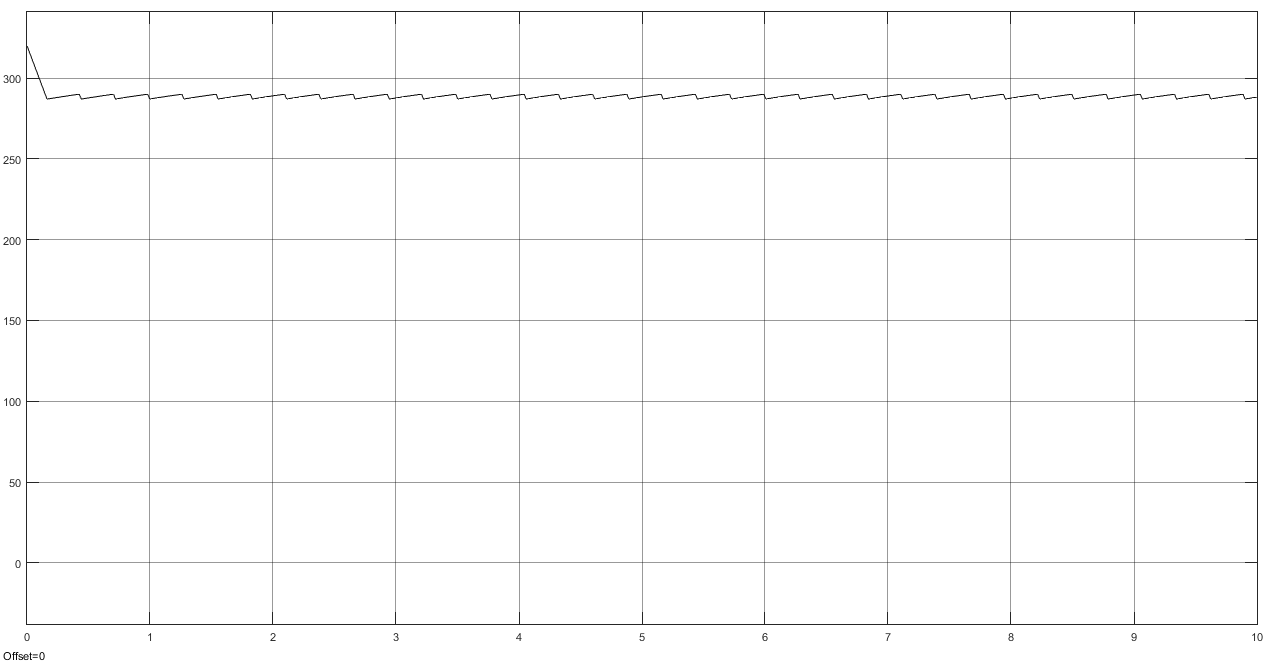
\includegraphics[width=.5\linewidth]{CicloLimiteTemp2.png}
\caption{a)Gráfico da temperatura para T(0)=250K b)Gráfico da temperatura para T(0)=320K}
\end{figure}

\begin{figure}[htpb!]
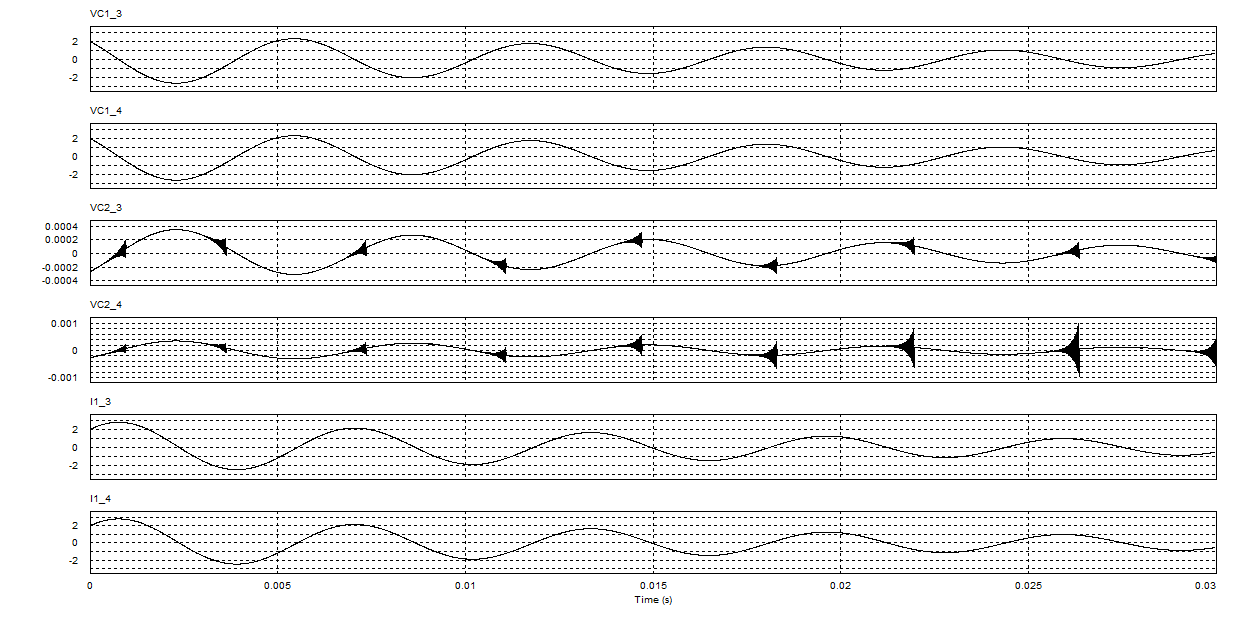
\includegraphics[width=.5\linewidth]{CaosBifurcBifVariaveis.png}
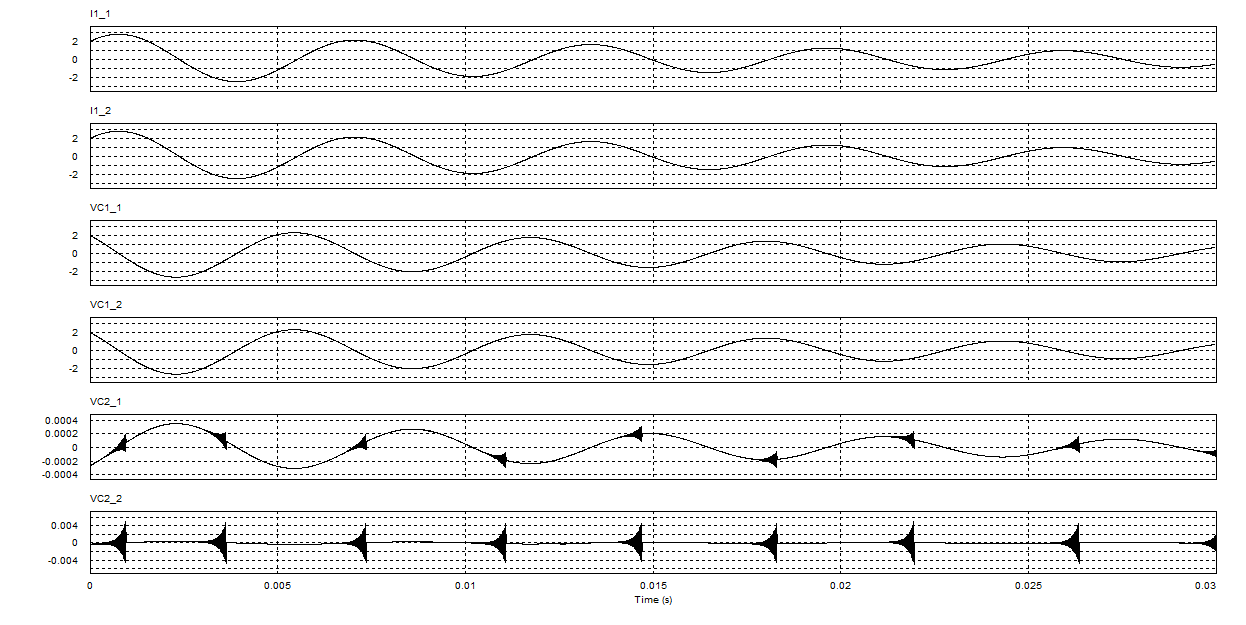
\includegraphics[width=.5\linewidth]{CaosBifurcCaoVariaveis.png}
\caption{a)Fenômeno da Bifurcação  b)Fenômeno do Caos}
\end{figure}


\begin{figure}[htpb!]
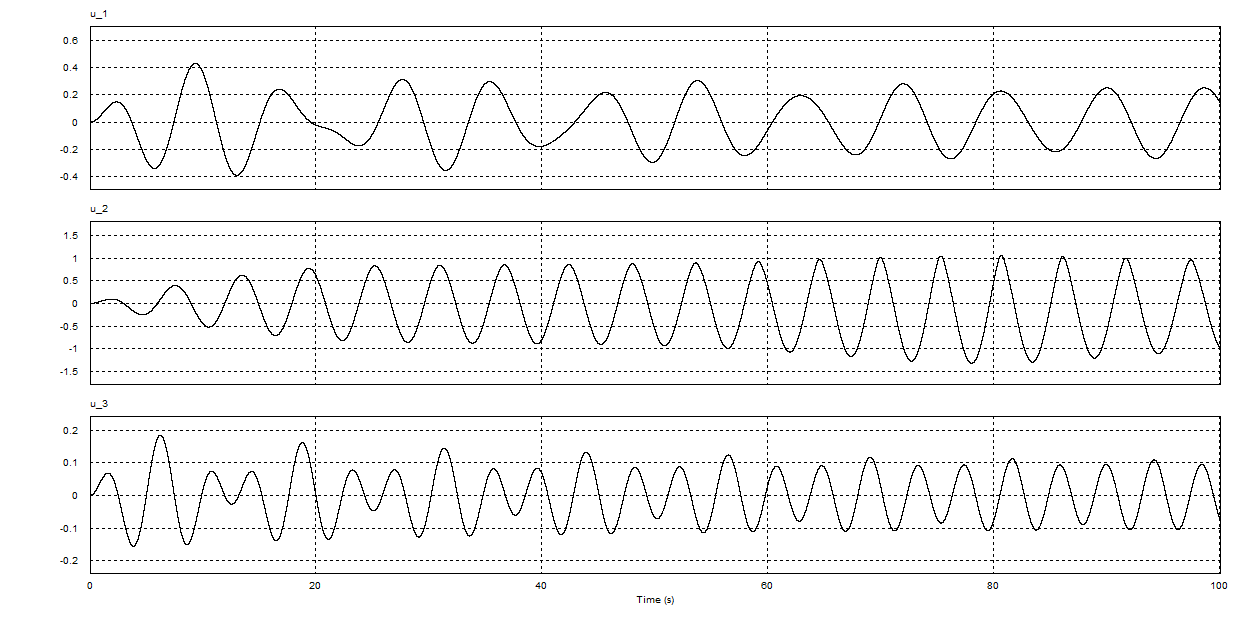
\includegraphics[width=\linewidth]{FenomenoSaltoVariaveis.png}
\caption{Saída do sistema para $\Omega_1=0.7, \Omega_2=1.1$ e $\Omega_3=1.5$ respectivamente}
\end{figure}



 \begin{figure}[htpb!]
 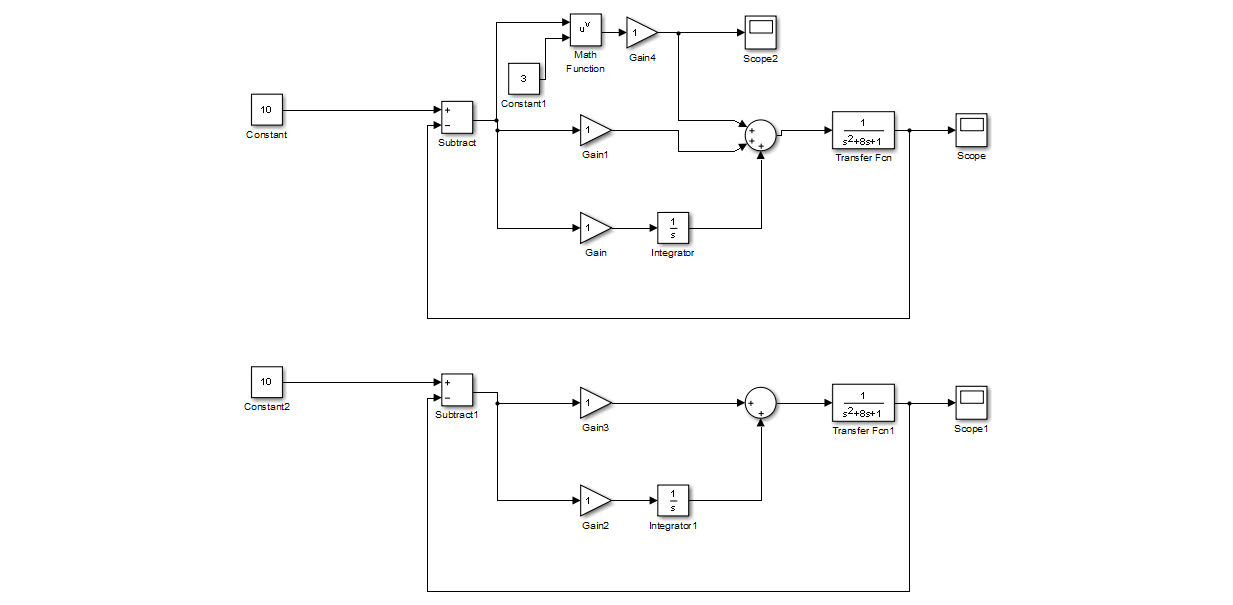
\includegraphics[width=.5\linewidth]{PInLinearEsquema.png}
 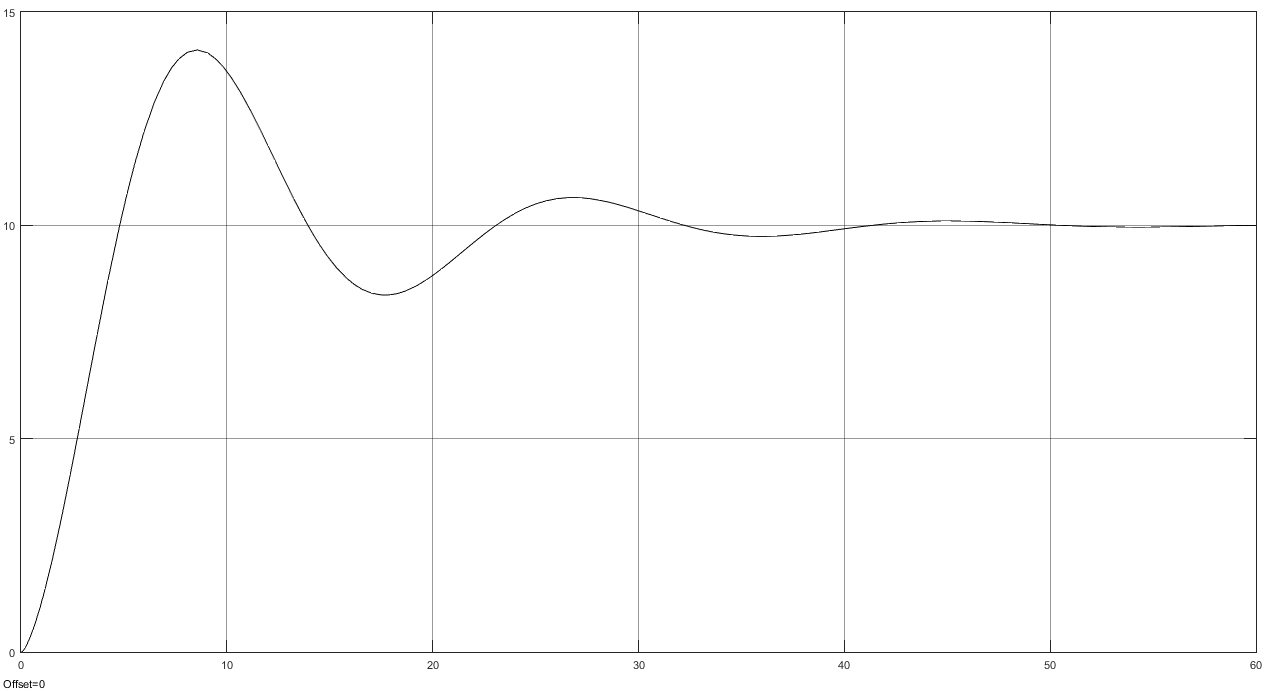
\includegraphics[width=.5\linewidth]{PInLinearRespostaLinear.png}
  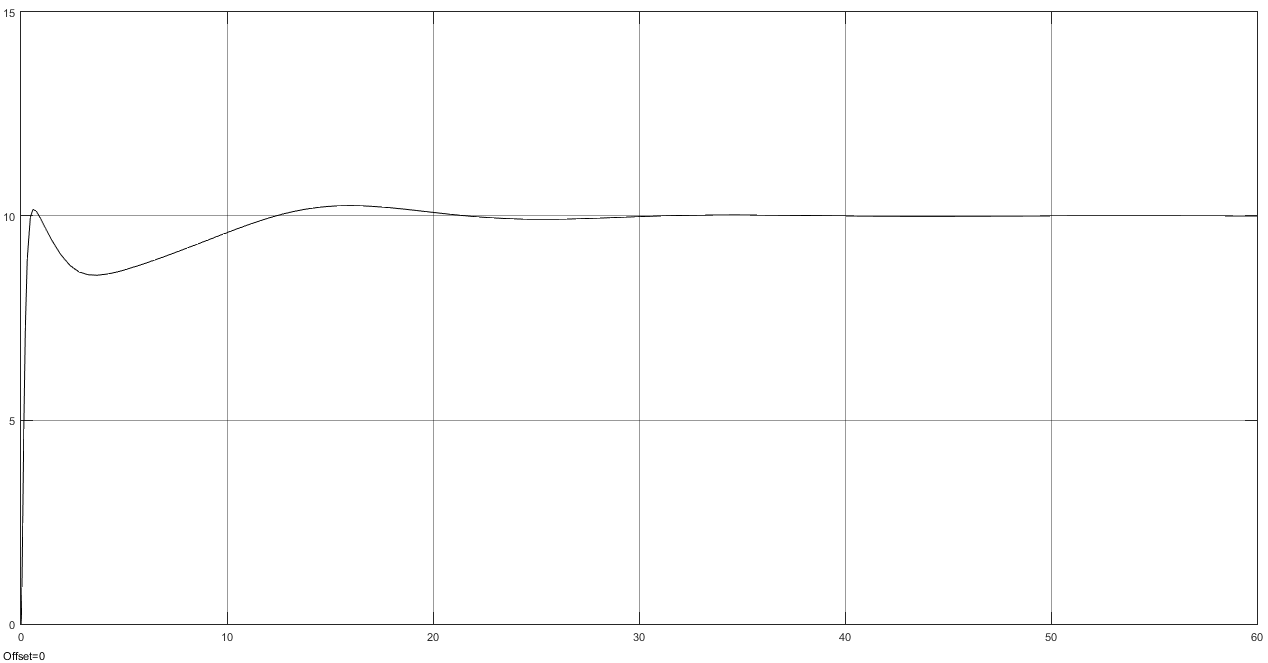
\includegraphics[width=.5\linewidth]{PInLinearResposta.png}
   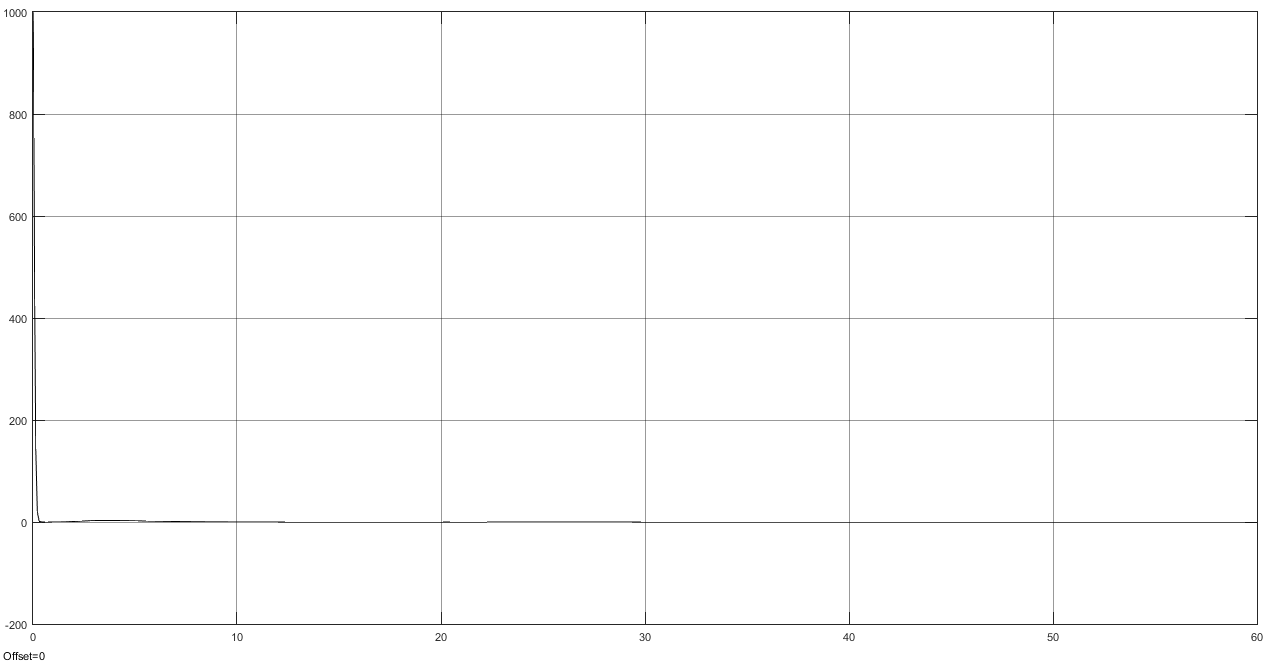
\includegraphics[width=.5\linewidth]{PInLinearCuboErro.png}
   \caption{a)Esquema usado para representar os dois controladores  b)Saída da planta para PI linear c)Saída da planta para PI não linear  d)Termo não linear introduzido}
   \end{figure}
   
   
   
     \begin{figure}[htpb!]
     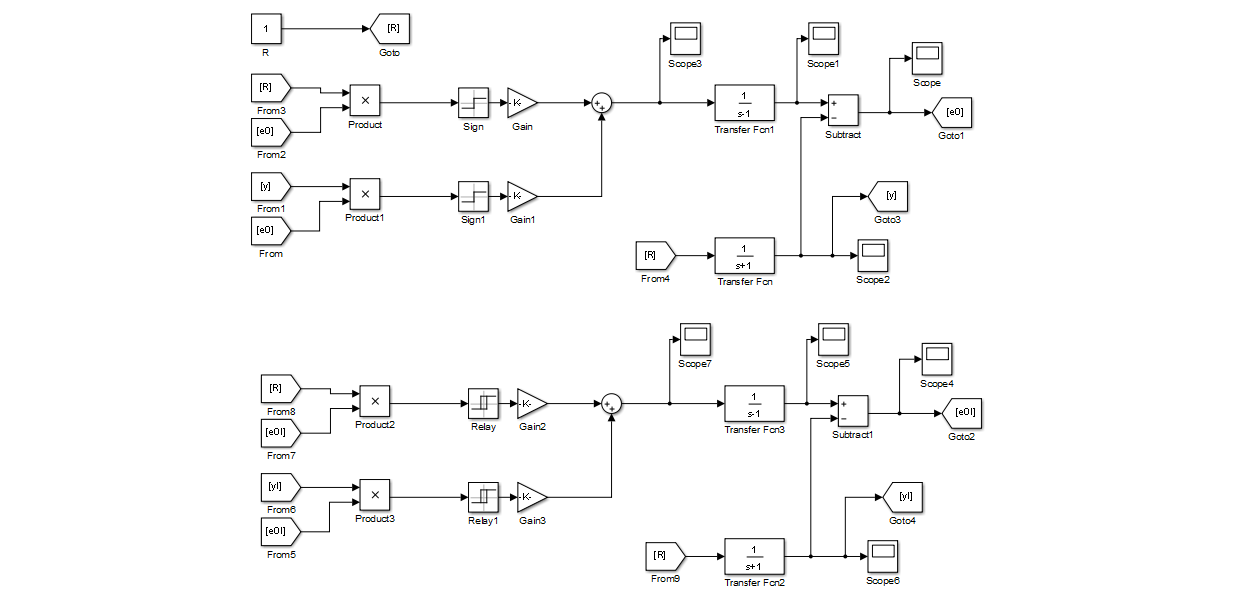
\includegraphics[width=.5\linewidth]{ControleReleVSEsquema.png}
       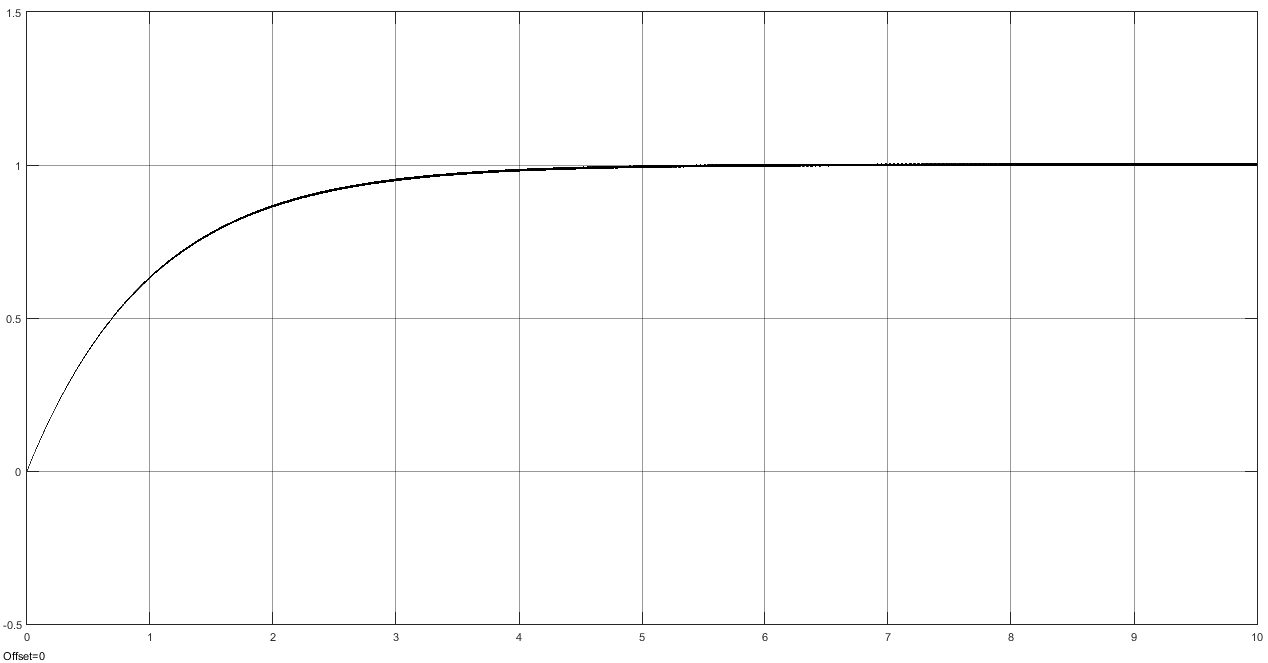
\includegraphics[width=.5\linewidth]{ControleReleVSSaidaSemHisterese.png}
           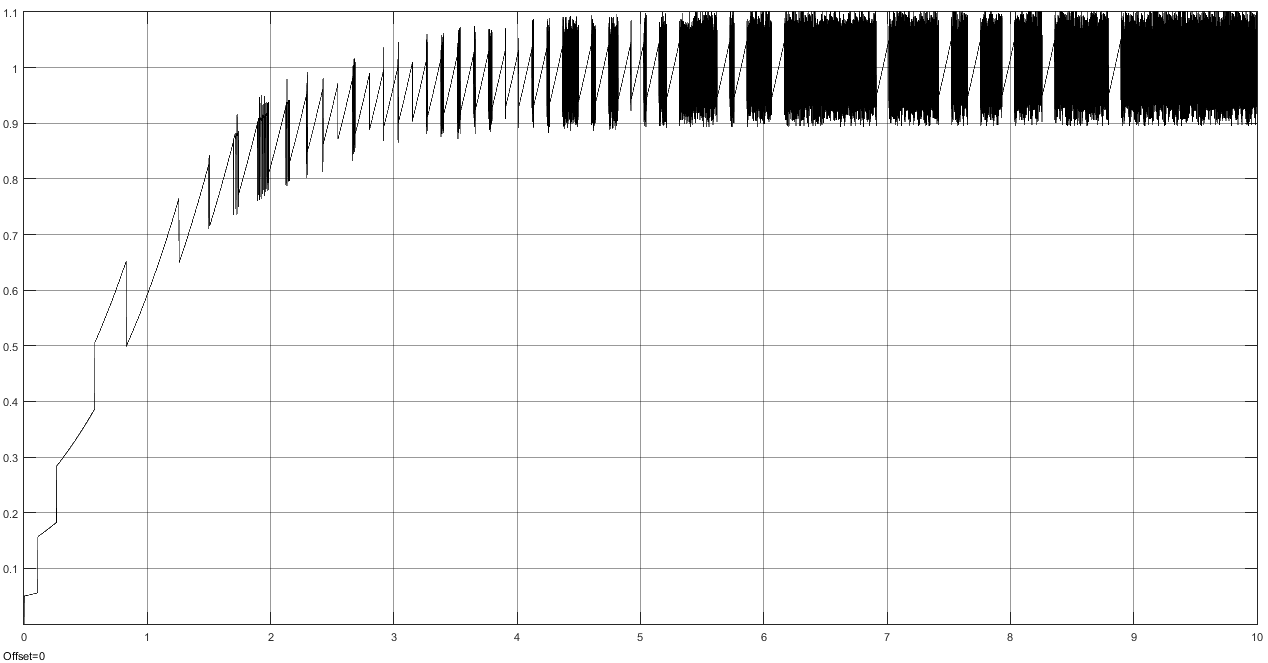
\includegraphics[width=.5\linewidth]{ControleReleVSSaidaComHisterese.png}
           \caption{a)Esquemas do controlador VS dado em aula com e sem histerese  b)Saída da planta para um controlador VS sem histerese c) Saída da planta para um controlador VS com histerese, +1 para entrada maior que 0.05 e -1 para entrada menor que -0.05}
           \end{figure} 
           
           
           
           \begin{figure}[htpb!]
           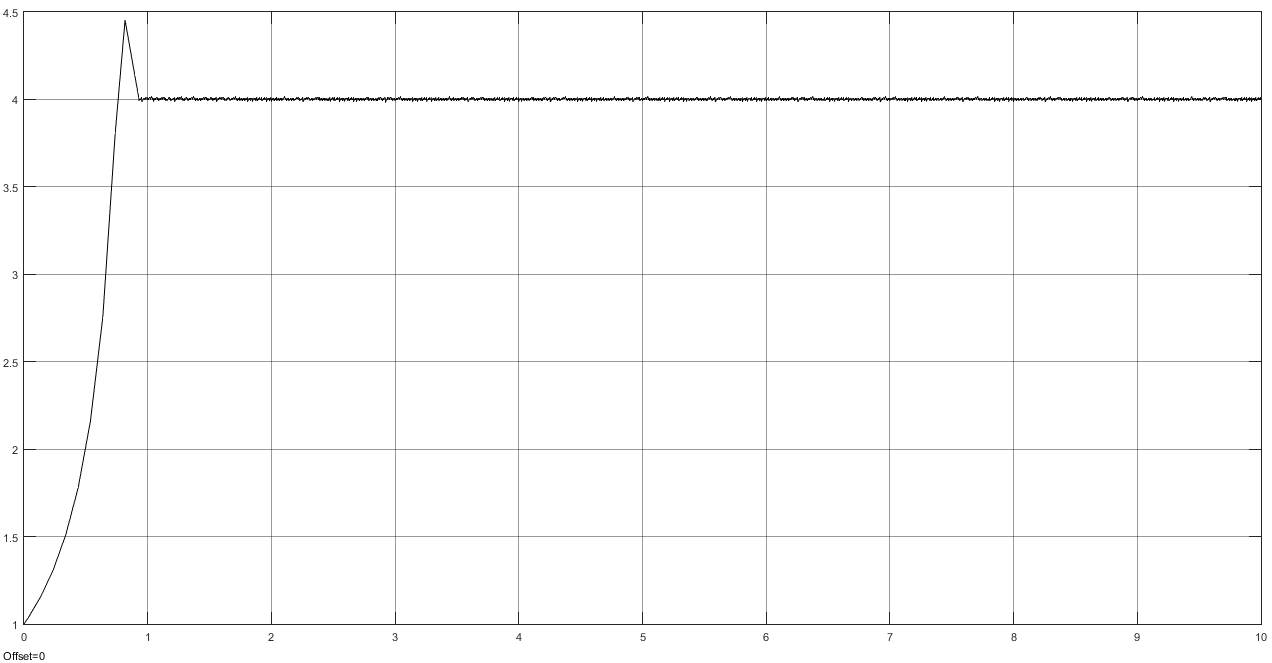
\includegraphics[width=.5\linewidth]{LipschitzLocal1.png}
           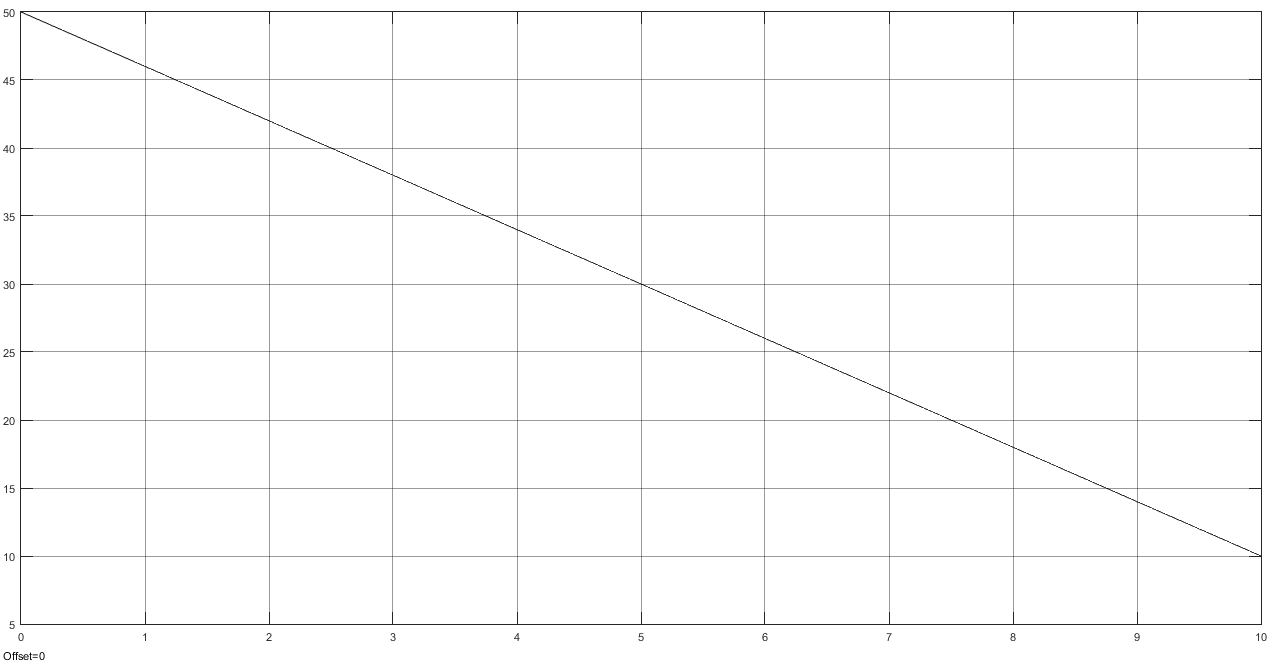
\includegraphics[width=.5\linewidth]{LipschitzLocal2.png}
           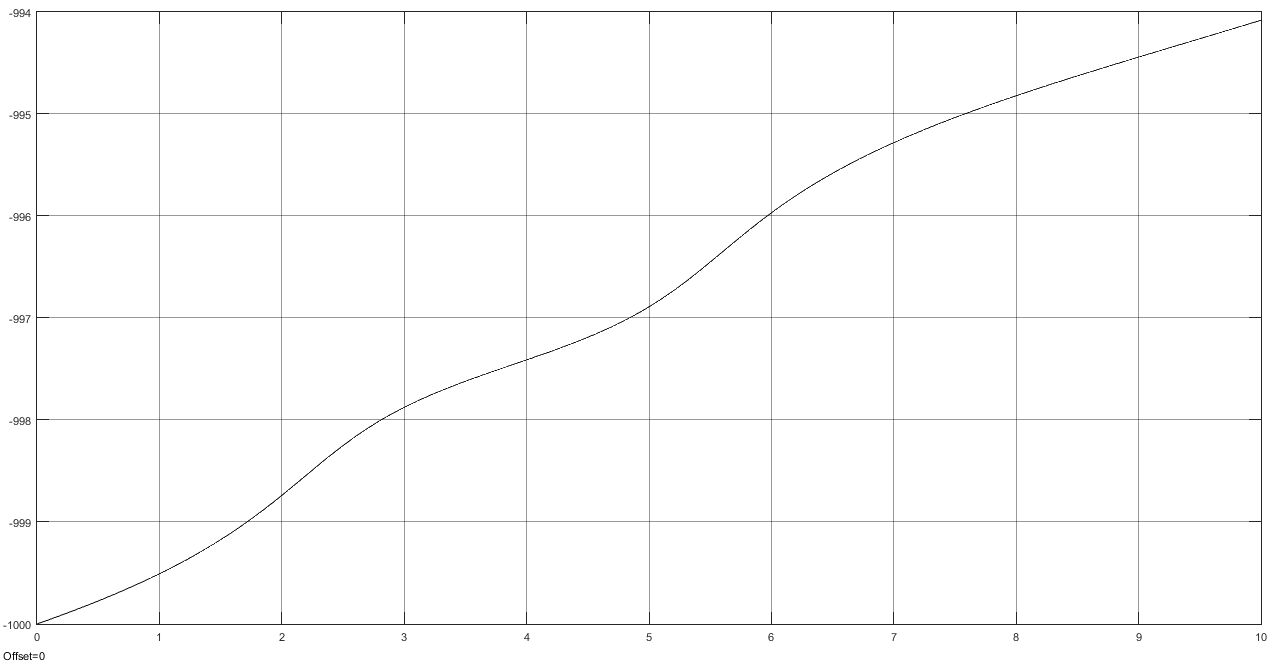
\includegraphics[width=.5\linewidth]{LipschitzGlobal1.png}
           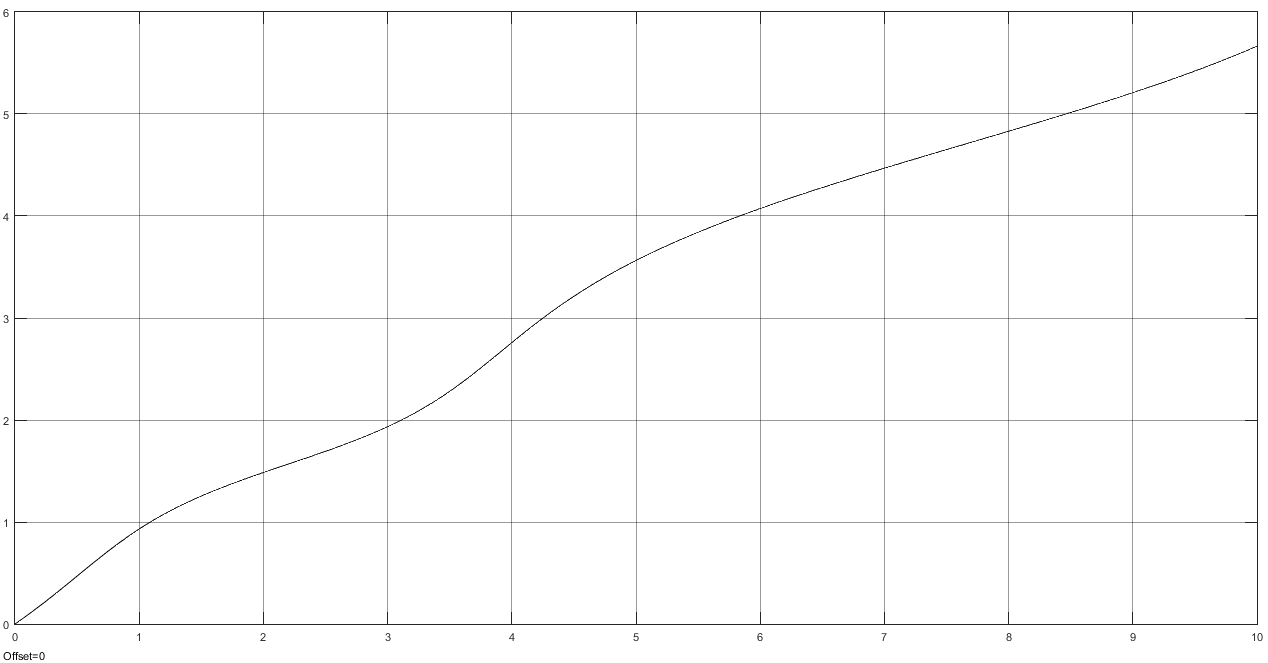
\includegraphics[width=.5\linewidth]{LipschitzGlobal2.png}
           \caption{a)Equação Lipschitz local simulada para condição inicial u(0)=1, o sistema tem soluções distintas para u maior que 4 e u menor que 4 b) Equação Lipschitz local simulada para condição inicial u(0)=50 c)Equação Lipschitz global simulada para condição inicial u(0)=0 d)Equação Lipschitz local simulada para condição inicial u(0)=-1000, o sistema possui a mesma solução nas duas regiões}
           \end{figure} 
           


\end{document}         